\documentclass[12pt]{article}
\usepackage{listings}
\usepackage{xcolor}
\usepackage{pgf-umlsd}
\usepackage{hyperref}
\usepackage{graphicx}
\graphicspath{ {./} }

\usepackage{tabularx}
\newcolumntype{b}{X}
\newcolumntype{s}{>{\hsize=.5\hsize}X}

\definecolor{codegreen}{rgb}{0,0.6,0}
\definecolor{codegray}{rgb}{0.5,0.5,0.5}
\definecolor{codepurple}{rgb}{0.58,0,0.82}
\definecolor{backcolour}{rgb}{0.95,0.95,0.92}
\lstdefinestyle{mystyle}{
    backgroundcolor=\color{backcolour},
    commentstyle=\color{codegreen},
    keywordstyle=\color{magenta},
    numberstyle=\tiny\color{codegray},
    stringstyle=\color{codepurple},
    basicstyle=\ttfamily\footnotesize,
    breakatwhitespace=false,
    breaklines=true,
    captionpos=b,
    keepspaces=true,
    numbers=left,
    numbersep=5pt,
    showspaces=false,
    showstringspaces=false,
    showtabs=false,
    tabsize=2
}
\lstset{style=mystyle}

\title{Emulation Framework for AIoT Federated Learning}
\author{Brendan Ang Wei Jie}
\begin{document}

\maketitle

\pagebreak
\section{Abstract}
Federated learning allows a fleet of devices to collaborate towards a globally trained machine
learning model. Research has continued to produce novel federated learning algorithms to tackle
different issues in FL such as heterogeneity and learning over data from non-identical
distributions. Performance of these algorithms depend in part on the system parameters used in FL
such as number of clients and number of passes. Furthermore, a realistic benchmark would require
one to procure a large fleet of devices. This work seeks to introduce a software emulation framework to
streamline the process of building a fleet of clients and allow easy testing of FL system
parameters for configuration of optimal values.
\pagebreak
  \section{Acknowledgements}
\pagebreak
\tableofcontents
\listoffigures
\pagebreak

\section{Introduction}
Federated learning emerged as a method for solving key issues with the standard centralized learning
approach. Some of these issues are (1) Preserving user data privacy: a centralized training approach involves the need for the central
machine performing the computation to have full access to all the data. With FL, data never
leaves each individual client's device. Instead, only the updated weights are shared to form the
global model.(2) Scalability: FL enables leveraging a network to perform computation in parallel.
\\
The distributed nature of FL poses a few key challenges. Some of these include:
\begin{itemize}
  \item Limited computing resources: individual devices may have constraints on memory, limiting the
    size of the local model it is able to train. Constraints on computing power can also lead to
    longer training times. This is particularly so for Internet of Things (IoT) devices such as
    sensors, where their embedded nature leads to a limited size and power.
  \item Network limitations: communication speed can become the bottleneck for performance as IoT
    devices rely on unstable wireless communication networks. Furthermore, data constraints can
    exist such that the number of bytes sent may be a cost inducing factor.
\end{itemize}

Hence, development of FL algorithms often seek to advance progress towards solving these
aforementioned issues.

\subsection{Problem}
However, prior to effectively deploying FL, different factors including the convergence rate and
model accuracy needs to be well studied, giving rise to the need for simulation. In addition, the
simulation of FL in the distributed setting involves dealing with
issues which do not arise in datacenter ML research. These include running on different simulated
devices each with potentially varying amount of data. Furthermore, metrics such as number of bytes uploaded and
downloaded by the device as well as the ability to simulate real-world issues such as client
drop-out can also be important for proposed FL algorithms to handle.

\subsection{Literary Review}
FedML\cite{} is a research-oriented library which supports various algorithms and 3 platforms, on-device training for IoT and
mobile devices, distributed computing and single-machine simulation. On-device training is supported
only on Raspberry Pi 4 and NVIDIA Jetson Nano which limits hardware validation to these 2 devices.
Simulation is offered through the FedML Parrot\cite{}, which offers an accelerated simulation
framework employing multiple optimizations to improve simulation speed.

FLSim\cite{} aims to provide a simulation framework for FL by offering users a set of software components
which can then be mixed and matched to create a simulator for their use case. Developers need only
define the data, model and metrics reported, and FL system parameters can be altered in a JSON
configuration file. FLUTE\cite{} adds additional features by allowing users to gain access to cloud based
compute and data. However, these simulation solutions are consequently hardware-agnostic. Without
taking into account the specific platforms which FL is performed on, these simulators cannot provide
insight into whether the system will work in the production environment.

Here, this work proposes a new emulation framework zfl, which aims to achieve the following
properties:
\begin{itemize}
  \item Provide better insight into platform specific support by running FL on emulated hardware.
  \item Collect useful metrics during the FL lifecycle.
  \item Support implementation of real word issues such as variable data and client drop-off.
\end{itemize}

\subsection{QEMU}
QEMU\cite{} is an open source machine emulator and virtualizer. It enables system emulation, where it
provides a virtual model of an entire machine (CPU, memory and emulated devices) to run a guest OS.
In this mode the CPU may be fully emulated, or it may work with a hypervisor to allow the guest to
run directly on the host CPU. In zfl, QEMU with full CPU emulation is used without a hypervisor as
part of its software architecture to emulate hardware.

\subsection{Zephyr OS}
To emulate the issue of limited computing resources, it is important to make use of system runtimes
used by those devices. In particular, the type of operating system used will help to ensure that the kernel is
lightweight and configurable.
Zephyr OS\cite{} is one such OS. It is based on a small-footprint kernel designed for use on resource-constrained and embedded systems: from simple embedded environmental sensors and LED wearables to sophisticated embedded controllers, smart watches, and IoT wireless applications.
Furthermore, Zephyr is highly configurable, allowing the user to choose only the specific kernel
services required, and also delve into lower level memory allocations of the system RAM. In zfl,
client code will be written to work in the Zephyr OS environment.

\section{Implementation}
zfl aims to provide the ability to emulate the traditional FedAvg\cite{} algorithm, with multiple
clients communicating with a central server which performs the aggregation. To run on Zephyr OS, the entire software stack is developed in the C programming language. This also
makes it suitable to run on embedded devices.\\

Next the framework needed a method for spawning an arbitrary number of QEMU instances, and allowing
these instances to communicate back to the server. When called in client mode, zfl accomplishes this
by making use of the `fork` and `exec` pattern with the desired number of clients. \\

However, each instance of QEMU is persists in an isolated network different from the host PC,
and is not able to communicate. We can bypass this limitation using a network bridge to act as a
virtual network device forwarding packets between connected network devices.
The network bridge is set up on the host under the name zfl with a set of network parameters using
the \verb|ip| command line utility.
\begin{lstlisting}[language=bash,caption=Network bridge setup]
ip link add $INTERFACE type bridge
ip addr add $IPV4_ADDR_1 dev $INTERFACE
ip link set enp61s0 master $INTERFACE
ip route add $IPV4_ROUTE_1 dev $INTERFACE > /dev/null 2>&1
ip link set dev $INTERFACE up
\end{lstlisting}
To tell QEMU to use it, we pass the name of the bridge along
with a randomly generated MAC address as arguments to the -nic flag
\begin{verbatim}
  -nic bridge,model=e1000,mac=%s,br=zfl
\end{verbatim}

Although each QEMU client is now able to communicate with the host via the nic adapter, we still
needed a way to monitor the output of each instance. One method is to transmit
output and logs over the network. However, this would not allow important crash logs and stacktrace
information to be transmitted as the application software would have shutdown. To overcome this, the host
creates a named or FIFO pipe \cite{} for each client which is passed in to
QEMU through the -serial flag. Now, all standard output goes through the named pipe, ready to be read
by the host. Another outcome of this is that the host is now also able to send input to each
instance, whose importance will be described in the next section.

\begin{lstlisting}[language=C,caption=Client forking process]
pid_t child = fork();
if (child < 0) {
    printf("ERROR: could not fork client %d: %s\n", i, strerror(errno));
    return 1;
}
...

// generate serial arguments
char serial_arg[80];
snprintf(serial_arg, 80, "pipe:%s", pipe_path);

// generate nic arguments
char nic_arg[100];
char *mac = generate_random_mac();
snprintf(nic_arg, sizeof(nic_arg), "bridge,model=e1000,mac=%s,br=zfl", mac);

// start client as new process
execlp("qemu-system-i386", "qemu-system-i386",

       "-m", "15", "-cpu", "qemu32,+nx,+pae", "-machine", "q35",
       "-device", "isa-debug-exit,iobase=0xf4,iosize=0x04",

       "-no-reboot", "-nographic", "-no-acpi",

       "-serial", serial_arg,

       "-nic", nic_arg,

       "-kernel", "./zflclient/out/zephyr/zephyr.elf",

       NULL);
\end{lstlisting}

In addition to the MAC address configuration, each client needed a unique Internet Protocol Version
4 (IPv4) address in order to establish TCP based connections with the central server. Samples
provided by Zephyr OS describe a way to achieve this my setting a compile time configuration flag
\verb|CONFIG_NET_CONFIG_MY_IPV4_ADDR|. However, this is impractical to scale to a number of clients, since
each client would need a separately compiled binary. Instead, we can assign the IPv4 address
dynamically using the built-in Zephyr network function:
\begin{verbatim}
net_if_ipv4_addr_add
\end{verbatim}
To achieve this, each client starts off as a Zephyr shell instance and a user-defined command is registered as a way to start the main program.
The desired IP address is obtained using the command line argument in listing \ref{lst:shellcmd}.

\begin{lstlisting}[language=C, caption=Registering user defined command "run" to the function
pointer run,label={lst:shellcmd}]
SHELL_CMD_ARG_REGISTER(run, NULL, "Run with IPv4 address", run, 4, 0);
\end{lstlisting}

The complete architecture is illustrated in figure \ref{fig:architecture}.

\begin{lstlisting}[language=C, caption=the "run" function which performs IP address assignment at runtime]
    char *addr_str = argv[1];
    LOG_INF("instance ipaddr is %s", addr_str);
    struct in_addr addr;
    zsock_inet_pton(AF_INET, addr_str, &addr);
    if (!net_if_ipv4_addr_add(net_if_get_default(), &addr, NET_ADDR_MANUAL, UINT32_MAX)) {
        LOG_ERR("failed to add %s to interface", addr_str);
        return -1;
    }
\end{lstlisting}

\begin{figure}
  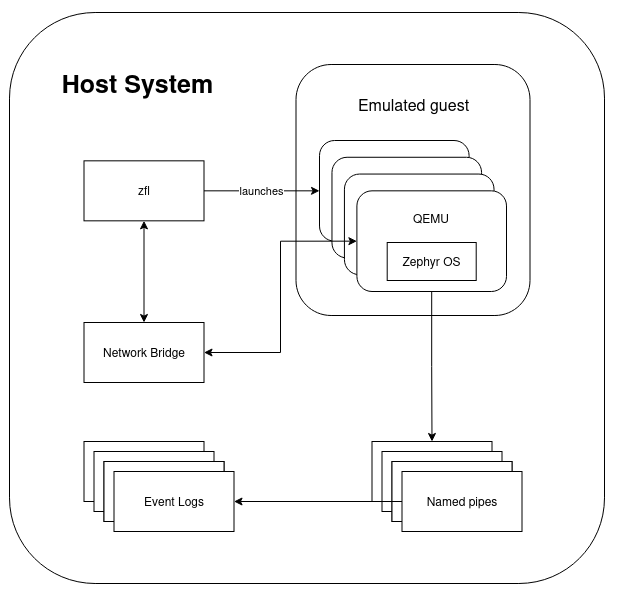
\includegraphics[scale=0.8]{architecture}
  \caption{Host-guest emulation architecture}
  \label{fig:architecture}
\centering
\end{figure}

\subsection{Client}
Each client establishes TCP socket connection to the central server and obtains
their assigned ID and training data according to that ID. Once done, each client
starts a HTTP server and marks itself as ready to begin the training round. The complete initialization process is
illustrated in figure \ref{fig:clientinit}.

\begin{figure}]
  \centering
  \begin{sequencediagram}
    \newthread{A}{Client}{}
    \newinst[1]{B}{Server}{}
    \begin{call}{A}{getId()}{B}{id}
    \end{call}
    \begin{call}{A}{getTrainingData(id)}{B}{data}
    \end{call}
    \begin{call}{A}{self.ready = true}{A}{}
    \end{call}
  \end{sequencediagram}
  \caption{Client initialization sequence}
  \label{fig:clientinit}
\end{figure}

\subsection{Server}
The central server runs on the host machine without needing additional configuration. Its primary
purpose is to serve as a HTTP server. Implemented endpoints are described in figure
\ref{fig:httpendpoints}. After assigning each connecting client their ID and training data, it performs the function
\verb|start_round| at an interval of 10 seconds. Each time, the server pings all previously
connected clients to check if they are ready to start the training round. When enough clients are
ready, it sends a HTTP post request to the \verb|train| endpoint of the client, which triggers the training
function. Once the client has completed training, it sends the resulting weights of the local model
to the HTTP POST endpoint \verb|results| of the server, who then performs the aggregation. The
sequence of events for a single round is illustrated in figure \ref{}.

\begin{figure}
\begin{tabularx}{\textwidth} {
  | >{\raggedright\arraybackslash}s
  | >{\centering\arraybackslash}s
  | >{\raggedright\arraybackslash}b | }
 \hline
 \multicolumn{3}{|c|}{Client} \\
 \hline
 Endpoint & HTTP Method & Description \\
 \hline
 /start & POST & Initiates training round using updated weights with JSON body: \newline\{weights: int\}  \\
 \hline
 /ready & GET & Gets client ready status \\
 \hline
 \multicolumn{3}{|c|}{Server} \\
 \hline
 /results?id= & POST & Client id submits results with JSON body: \newline\{round: int, weights: string\}  \\
 \hline
 /id & GET & Obtain an id for round participation \\
 \hline
 /training-data?id= & GET & Obtain training data for id \\
 \hline
 /training-labels?id= & GET & Obtain training labels for id \\
 \hline
\end{tabularx}
\caption{HTTP endpoints}
\label{fig:httpendpoints}
\end{figure}

\section{Experiments}
The framework is tested using FedAvg over the MNIST digit recognition data set. Due to memory
constraints, clients are configured with a neural network architecture with 1 hidden layer of 16
nodes. The underlying neural network implementation utilizes nn.h\cite{}, an open source educational neural network C
library. Additionally, implementations for the softmax activiation and cross entropy were made to
make it suitable for machine learning with MNIST categorical data.

\section{Limitations}
\subsection{Long training times}\
Unoptimized client training implementations has resulted in long training times required per FL
round. This is because we were unable to find standard implementations for machine learning
algorithms that can be easily ported for use in the Zephyr OS. Zephyr OS provides external modules
for supporting Tensorflow Lite Micro\cite{} and has examples for running pre-trained neural network
on their platform. However, on-device training is not supported\cite{}.

\end{document}
